\documentclass[12pt]{report}
\usepackage[pdftex]{graphicx}
%\usepackage[pdftrex/bookmarksnumbered=true]{hyperref}
\usepackage{hyperref}
\linespread{1.5}
\textwidth = 6in
\textheight = 9in
\usepackage[body={6.0in, 8.2in},left=1.25in,right=1.0in,top=1.0in, bottom=1.0in]{geometry}
\frenchspacing
\usepackage{fancyhdr}
\usepackage{color}
\usepackage{xcolor}
\usepackage{listings}
\lstset{
language=Java,
basicstyle=\small\sffamily,
numbers=left,
numberstyle=\tiny,
frame=tb,
columns=fullflexible,
showstringspaces=false
}

\usepackage{caption}
\DeclareCaptionFont{white}{\color{white}}
\DeclareCaptionFormat{listing}{\colorbox{gray}{\parbox{\textwidth}{#1#2#3}}}
\captionsetup[lstlisting]{format=listing,labelfont=white,textfont=white}


\begin{document}
\pagenumbering{roman}
%\input{Coverpage.tex}

%----------------title page
\begin{titlepage}
\begin{center}
{\bf \large Decision Tree Classifier with GA based feature selection}\\
\vspace{.15in}
{\bfseries Mini Project Report}\\
\vspace{.15in}
{\normalsize Submitted to} \\
\vspace{.1in}
{\bfseries DEPARTMENT OF COMPUTER SCIENCE AND ENGINEERING}\\
\vspace{.25in}
{\normalsize \emph{By}}\\
{\bfseries\normalsize Samir Sheriff }\\
{\bfseries\normalsize Satvik N }\\
\vspace{.25in}
{\normalsize \emph{In partial fulfilment of the requirements\\ for the award of the degree \\
\vspace{.15in}
} } 

\vspace{.15in}
{\large{BACHELOR OF ENGINEERING}}\\
\vspace{.15in}
{\normalsize{IN}}\\
\vspace{.15in}
{\bfseries\normalsize COMPUTER SCIENCE AND ENGINEERING}\\
\vspace{0.15in}

\begin{figure}[h!]
	\centering
		\includegraphics[scale=0.5]{RVCE.png}
		
\end{figure} 
\vspace{.25in}
{\bfseries\large R V College of Engineering}\\
{\normalsize (Autonomous Institute, Affiliated to VTU)}\\
{\bfseries\normalsize BANGALORE - 560059}\\ 
{\bfseries\large May 2012}
\end{center}
\end{titlepage}


%---------Declaration
\begin{titlepage}
%\chapter*{\centerline{DECLARATION}}
\begin{center}
\section*{DECLARATION}
\end{center}

\paragraph{}  We, Samir Sheriff and Satvik N bearing USN number 1RV09CS093 and 1RV09CS095 respectively, hereby declare that the dissertation entitled ``\textbf{Decision Tree Classifier with GA feature selection}'' completed and written by us, has not been previously formed the basis for the award of any degree or diploma or certificate of any other University.
\vspace{1in}

\begin{flushright} {Bangalore \hspace{4.4in} Samir Sheriff } 
 {USN:1RV09CS093}
 \end{flushright}

\begin{flushright} { Satvik N } \\
 {USN:1RV09CS095}
 \end{flushright}
\end{titlepage}

%---------Certificate
\begin{titlepage}
\newpage
\begin{center}
{\bfseries\large R V COLLEGE OF ENGINEERING}\\
{\normalsize (Autonomous Institute Affiliated to VTU)}\\
{\normalsize DEPARTMENT OF COMPUTER SCIENCE AND ENGINEERING}\\
\end{center}
	
\begin{figure}[h!]
	\centering
		\includegraphics[scale=0.5]{RVCE.png}
		%\includegraphics{msrit-logo.jpg}
	%\caption{}
	%\label{fig:logo2}
\end{figure}

\begin{center}
\bf{\underline{CERTIFICATE}}
\end{center}
\noindent This is to certify that the dissertation entitled, ``\textbf{Decision Tree Classifier with GA based feature selection}'',  which is being submitted herewith for the award of B.E is the result of the work completed by \textbf{Samir Sheriff and Satvik N}  under my supervision and guidance.
\vspace{.5in}

\begin{flushleft} Signature of Guide 	
\\ (Name of the Guide) \\
\vspace{.5in}
 Signature of Head of Department  \hspace{4cm} Signature of Principal \\
 (Dr. N K Srinath) \hspace{6.6cm} (Dr. B.S Sathyanarayana)\\
 
 \end{flushleft} 
\begin{flushleft}
\hspace{1in}Name of Examiner \hspace{1.25in} Signature of Examiner
\end{flushleft}
\begin{flushleft}
1: \\
\vspace{.5in} 
2: 
\end{flushleft}
\end{titlepage}


%---------Acknowledgement
  
%\linespread{1.5}
\setcounter{page}{1}
\begin{center}
\section*{ACKNOWLEDGEMENT}
\addcontentsline{toc}{section}{ACKNOWLEDGEMENT}
\end{center}
The euphoria and satisfaction of the completion of the project will be incomplete
without thanking the persons responsible for this venture.


We acknowledge RVCE (Autonomous under VTU) for providing an opportunity to
create a mini-project in the 5th semester. We express our gratitude towards \textbf{Prof. B.S. Satyanarayana}, principal, R.V.C.E for constant encouragement and facilitates extended in completion of this project. We would like to thank \textbf{Prof. N.K.Srinath}, HOD, CSE
Dept. for providing excellent lab facilites for the completion of the project. We would
personally like to thank our project guides \textbf{Ms. Shantha Rangaswamy and Dr. G. Shobha} and also the lab in charge, for providing timely assistance \& guidance at the time.



We are indebted to the co-operation given by the lab administrators and lab assistants,
who have played a major role in bringing out the mini-project in the present form.
Bangalore



\begin{flushright}
Samir Sheriff\\
7th semester, CSE\\
USN:1RV09CS093\\

Satvik N\\
7th semester, CSE\\
USN:1RV09CS095\\

\end{flushright}

\newpage

%--------------Abstract
%\fontfamily{roman}%\selectfont
\begin{center}
\section*{ABSTRACT}
\addcontentsline{toc}{section}{ABSTRACT}
\end{center} 
Machine Learning techniques have been applied to the field of classification for more than a decade. Machine Learning techniques can learn normal and anomalous patterns from training data and generate classifiers, which
can be used to capture characteristics of interest. In general, the input data to classifiers is an extremely large set of features, but not all of features are relevant to the classes to be classified.
Hence, the learner must generalize from the given examples in order to produce a useful output in new cases. 

A major focus of machine learning research is the design of algorithms that recognize complex patterns and make intelligent decisions based on input data. Our Project, titled ``\textbf{Decision Tree Classifier with Genetic Algorithm-based Feature Selection}” is aimed at developing a complete program that constructs an optimal decision tree, based on any kind of data set, divided into training and testing examples, by selecting only a subset of features to classify data. 

Although our program works with generic data samples, it must be noted that when we started this project, our main intention was to classify ground water samples into two classes, namely Potable and Non-Potable Water. However, thanks to the miracle of Object-Oriented Programming Concepts, we were able to extend this project.



%------Table Of Contents
\addcontentsline{toc}{section}{CONTENTS}
\tableofcontents
%\listoffigures
%\listoftables


\newpage

\pagenumbering{arabic}
\setcounter{page}{1}

\pagestyle{fancy}
\lhead{\scriptsize{Introduction}}
\chead{}
\rhead{\scriptsize{DT Classifier with GA based feature selector.}}
\lfoot{\scriptsize{Dept. of CSE, RVCE, Bangalore.}}
\rfoot{\small{\thepage}}
\cfoot{\scriptsize{Sept 2012 - Jan 2013}}
\renewcommand{\headrulewidth}{0.4pt}
\renewcommand{\footrulewidth}{0.4pt}

\chapter{INTRODUCTION}


Machine learning, a branch of artificial intelligence, is about the construction and study of systems that can learn from data. The core of machine learning deals with representation and generalization. Representation of data instances and functions evaluated on these instances are part of all machine learning systems. There is a wide variety of machine learning tasks and successful applications. 






\section{SCOPE}

The machine learning concepts we have used in our project are listed below,
\begin{itemize}


\item{\textbf{Supervised learning}}  is the machine learning task of inferring a function from labeled training data. The training data consist of a set of training examples. In supervised learning, each example is a pair consisting of an input object (typically a vector) and a desired output value (also called the supervisory signal). A supervised learning algorithm analyzes the training data and produces an inferred function, which is called a classifier (if the output is discrete; see classification) or a regression function (if the output is continuous; see regression). The inferred function should predict the correct output value for any valid input object. This requires the learning algorithm to generalize from the training data to unseen situations in a "reasonable" way.

\item{\textbf{Decision tree learning}}, used in statistics, data mining and machine learning, uses a decision tree as a predictive model which maps observations about an item to conclusions about the item's target value. The goal is to create a model that predicts the value of a target variable based on several input variables.

\item A {\textbf{Genetic Algorithms}} is a search heuristic that mimics the process of natural evolution. This heuristic is routinely used to generate useful solutions to optimization and search problems. Genetic algorithms belong to the larger class of evolutionary algorithms (EA), which generate solutions to optimization problems using techniques inspired by natural evolution, such as inheritance, mutation, selection, and crossover.

\end{itemize}


\pagestyle{fancy}
\lhead{\scriptsize{Software Requirements Specification}}
\chead{}
\rhead{\scriptsize{Decision Tree Classifier with GA-based Feature Selection}}
\lfoot{\scriptsize{Dept. of CSE, R V C E, Bangalore.}}
\rfoot{\small{\thepage}}
\cfoot{\scriptsize{Sept 2012 - Jan 2013}}
\renewcommand{\headrulewidth}{0.4pt}
\renewcommand{\footrulewidth}{0.4pt}
\chapter{REQUIREMENT SPECIFICATION}
Software Requirement Specification (SRS) is an important part of the  software development process. We describe the overall description of the Mini-Project, the specific requirements of the Mini-Project, the software requirements and hardware requirements and the functionality of the system.

\subsubsection{Software Requirements}
\begin{itemize}

\item{	Front End: Java SWT Application.}
\item{	Back End: Java}
\item{	Operating System: Windows 7, Ubuntu 12.10.}

\end{itemize}

\subsubsection{Hardware Requirements}
\begin{itemize}
\item{Processor: Intel Core 2 Duo or higher version}
\item{RAM: 4GB or more}
\item{Hard disk: 5 GB or less}
\end{itemize}

%\input{IMP.tex}
\pagestyle{fancy}
\lhead{\scriptsize{Decision Tree Learning}}
\chead{}
\rhead{\scriptsize{Decision Tree Classifier with GA-based Feature Selection}}
\lfoot{\scriptsize{Dept. of CSE, RVCE, Bangalore.}}
\rfoot{\small{\thepage}}
\cfoot{\scriptsize{Sept 2012 - Jan 2013}}
\renewcommand{\headrulewidth}{0.4pt}
\renewcommand{\footrulewidth}{0.4pt}
\chapter{Decision Tree Learning}

\section{Definition}


Decision tree is the learning of decision tree from class labeled training tuples. A decision tree is a flow chart like structure, where each internal (non-leaf) node denotes a test on an attribute, each branch represents an outcome of the test, and each leaf (or terminal) node holds a class label. The topmost node in tree is the root node.

There are many specific decision-tree algorithms. Notable ones include:

\begin{itemize}
\item{\textbf{ID3} (Iterative Dichotomiser 3)}
\item{\textbf{C4.5} algorithm, successor of ID3}
\item{\textbf{CART} (Classification And Regression Tree)}
\item{\textbf{CHi-squared Automatic Interaction Detector }(CHAID). Performs multi-level splits when computing classification trees.}
\item{\textbf{MARS}: extends decision trees to better handle numerical data}
\end{itemize}


\section{The Basic Idea}

Decision tree is a classifier in the form of a tree structure (as shown in Fig. 3.1, where each node is either:
\begin{enumerate}
\item{A \textbf{leaf node} - indicates the value of the target attribute (class) of examples} (\textit{In Fig. 3.1, the nodes containing values K=x, K=y)}
\item{A \textbf{decision node} - specifies some test to be carried out on a single attribute-value, with one branch and sub-tree for each possible outcome of the test.\textit{In Fig. 3.1, the nodes containing attributes A, B and C)}}

\end{enumerate}

\begin{figure}[h!]
	\centering
		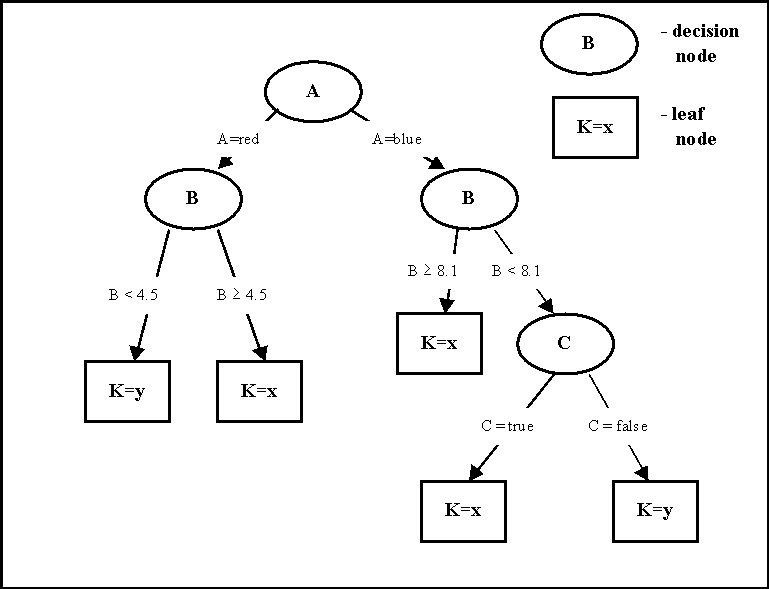
\includegraphics[scale=1.0]{dtreeexample.jpg}
	\caption{Sample Decision Tree}
	\label{fig:logo2}
\end{figure}

A decision tree can be used to classify an example by starting at the root of the tree and moving through it until a leaf node, which provides the classification of the instance.\\

Decision tree induction is a typical inductive approach to learn knowledge on classification. The key requirements to do mining with decision trees are:
\begin{itemize}
\item{\textbf{Attribute-value description}: object or case must be expressible in terms of a fixed collection of properties or attributes. This means that we need to discretize continuous attributes, or this must have been provided in the algorithm.\textit{(A, B and C, in Fig. 3.1)}}
\item{\textbf{Predefined classes (target attribute values)}: The categories to which examples are to be assigned must have been established beforehand (supervised data) \textit{(Classes X and Y in Fig. 3.1)}.}
\item{\textbf{Discrete classes}: A case does or does not belong to a particular class, and there must be more cases than classes.}
\item{\textbf{Sufficient data}: Usually hundreds or even thousands of training cases.}

\end{itemize}



\section{Building the Decision Tree}

Most algorithms that have been developed for learning decision trees are variations on a core algorithm that employs a top-down, greedy search through the space of possible decision trees. Decision tree programs construct a decision tree T from a set of training cases.


\subsection{ID3 Algorithm}
J. Ross Quinlan originally developed ID3 at the University of Sydney. He first presented ID3 in 1975 in a book, Machine Learning, vol. 1, no. 1. ID3 is based on the Concept Learning System (CLS) algorithm. ID3 searches through the attributes of the training instances and extracts the attribute that best separates the given examples. If the attribute perfectly classifies the training sets then ID3 stops; otherwise it recursively operates on the m (where m = number of possible values of an attribute) partitioned subsets to get their "best" attribute. The algorithm uses a greedy search, that is, it picks the best attribute and never looks back to reconsider earlier choices. Note that ID3 may misclassify data. 


\begin{figure}[h!]
	\centering
		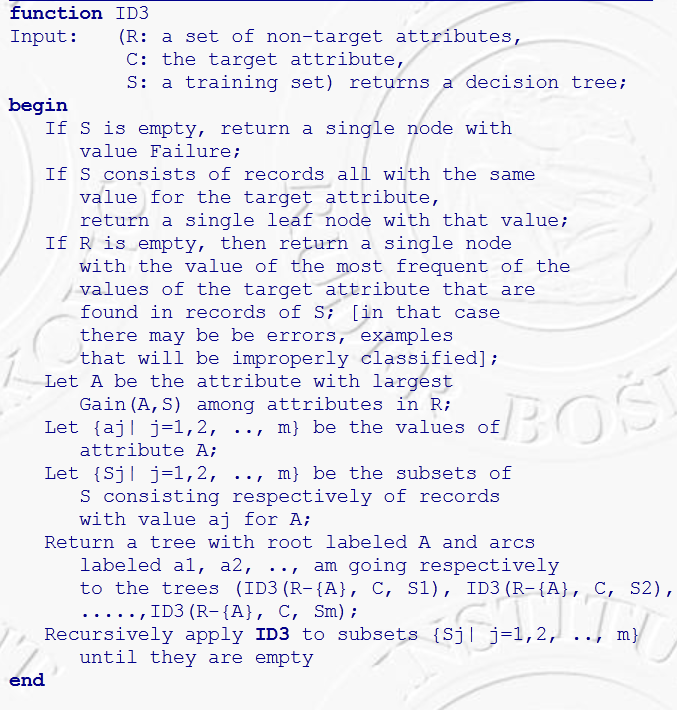
\includegraphics[scale=1.0]{ID3.png}
	\caption{ID3 Algorithm}
	\label{fig:ID3}
\end{figure}




\subsection{Choosing the best attribute for a given node}
The estimation criterion in the decision tree algorithm is the selection of an attribute to test at each decision node in the tree. The goal is to select the attribute that is most useful for classifying examples. A good quantitative measure of the worth of an attribute is a statistical property called information gain that measures how well a given attribute separates the training examples according to their target classification. This measure is used to select among the candidate attributes at each step while growing the tree. 

\subsection{Entropy - a measure of homogeneity of the set of examples}

In order to define information gain precisely, we need to define a measure commonly used in information theory, called entropy, that characterizes the (im)purity of an arbitrary collection of examples. Given a set S, containing only positive and negative examples of some target concept (a 2 class problem), the entropy of set S relative to this simple, binary classification is defined as:

\begin{math} Entropy(S) =  - p_{p}log_{2} p_{p} - p_{n}log_{2} p_{n} 
\end{math}

where p$_{p}$ is the proportion of positive examples in S and p$_{n}$ is the proportion of negative examples in S. In all calculations involving entropy we define 0 log 0 to be 0. 

To illustrate, suppose S is a collection of 25 examples, including 15 positive and 10 negative examples [15+, 10-]. Then the entropy of S relative to this classification is 

\begin{math} Entropy(S) = - (15/25) log_{2} (15/25) - (10/25) log_{2} (10/25) = 0.970 \end{math}


Notice that the entropy is 0 if all members of S belong to the same class. For example, if all members are positive (p$_{p}$= 1 ), then p$_{n}$ is 0, and:

\begin{math}Entropy(S) = -1 log_{2}(1) - 0 log_{2}0 = -1 0 - 0 log_{2}0 = 0. \end{math}

Note the entropy is 1 (at its maximum!) when the collection contains an equal number of positive and negative examples. If the collection contains unequal numbers of positive and negative examples, the entropy is between 0 and 1. Figure 3.3 shows the form of the entropy function relative to a binary classification, as p+ varies between 0 and 1. 


\begin{figure}[h!]
	\centering
		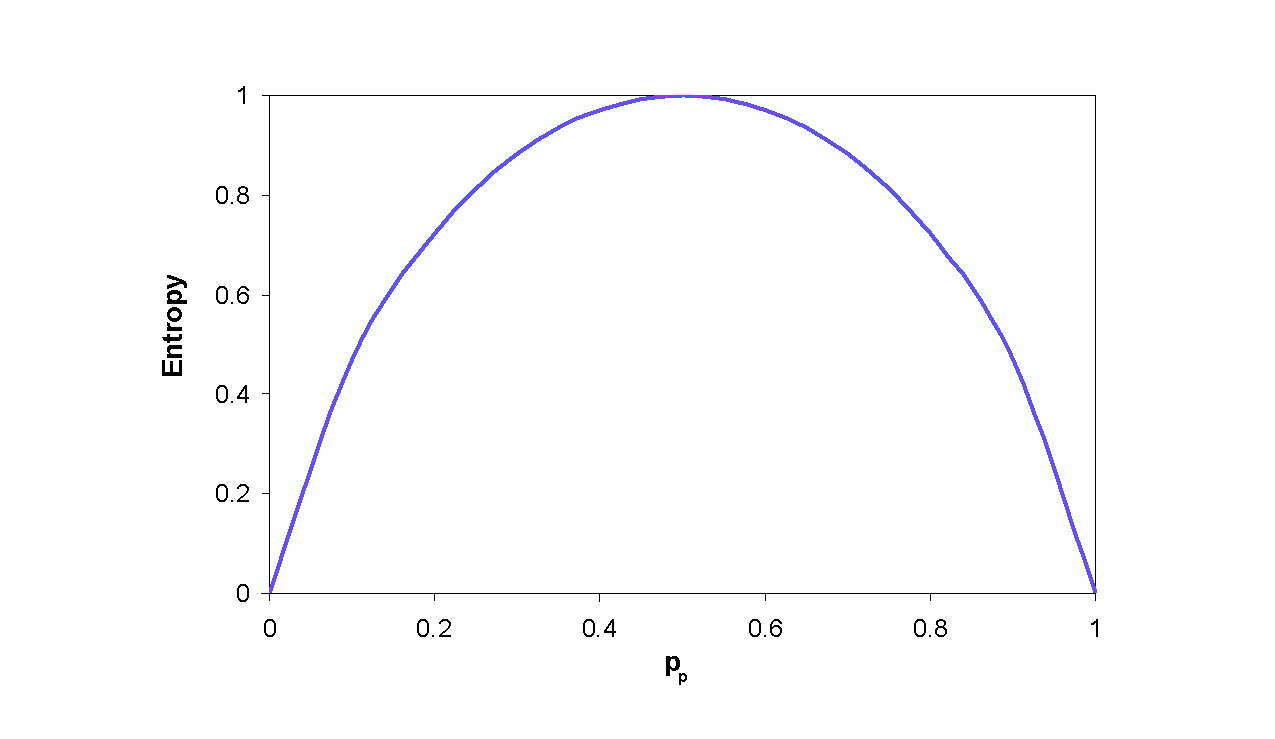
\includegraphics[scale=0.5]{entropy_graph.jpg}
	\caption{The entropy function relative to a binary classification, as the proportion of positive examples p$_{p}$ varies between 0 and 1.}
	\label{fig:ID3}
\end{figure}




One interpretation of entropy from information theory is that it specifies the minimum number of bits of information needed to encode the classification of an arbitrary member of S (i.e., a member of S drawn at random with uniform probability). For example, if p$_{p}$ is 1, the receiver knows the drawn example will be positive, so no message need be sent, and the entropy is 0. On the other hand, if p$_{p}$ is 0.5, one bit is required to indicate whether the drawn example is positive or negative. If p$_{p}$ is 0.8, then a collection of messages can be encoded using on average less than 1 bit per message by assigning shorter codes to collections of positive examples and longer codes to less likely negative examples.

Thus far we have discussed entropy in the special case where the target classification is binary. If the target attribute takes on c different values, then the entropy of S relative to this c-wise classification is defined as:

\begin{math}
Entropy(S) = \sum_{1}^{c} -p_{i} log_{2} p_{i}
\end{math}

where p$_{i}$ is the proportion of S belonging to class i. Note the logarithm is still base 2 because entropy is a measure of the expected encoding length measured in bits. Note also that if the target attribute can take on c possible values, the maximum possible entropy is log$_{2}$c. 

\subsection{Information gain measures the expected reduction in entropy}
Given entropy as a measure of the impurity in a collection of training examples, we can now define a measure of the effectiveness of an attribute in classifying the training data. The measure we will use, called information gain, is simply the expected reduction in entropy caused by partitioning the examples according to this attribute. More precisely, the information gain, Gain (S, A) of an attribute A, relative to a collection of examples S, is defined as:

\begin{math}
Gain(S, A) = Entropy(S) - \sum_{v \in Value(A)} \frac{S_{v}}{S} Entropy(S_{v})
\end{math}

where Values(A) is the set of all possible values for attribute A, and S$_{v}$ is the subset of S for which attribute A has value v (i.e., S$_{v}$ = {s Î S | A(s) = v}). Note the first term in the equation for Gain is just the entropy of the original collection S and the second term is the expected value of the entropy after S is partitioned using attribute A. The expected entropy described by this second term is simply the sum of the entropies of each subset S$_{v}$, weighted by the fraction of examples $|$S$_{v}$ $|$/$|S|$ that belong to S$_{v}$. Gain (S,A) is therefore the expected reduction in entropy caused by knowing the value of attribute A. Put another way, Gain(S,A) is the information provided about the target attribute value, given the value of some other attribute A. The value of Gain(S,A) is the number of bits saved when encoding the target value of an arbitrary member of S, by knowing the value of attribute A.

The process of selecting a new attribute and partitioning the training examples is now repeated for each non-terminal descendant node, this time using only the training examples associated with that node. Attributes that have been incorporated higher in the tree are excluded, so that any given attribute can appear at most once along any path through the tree. This process continues for each new leaf node until either of two conditions is met:

\begin{enumerate}
\item{Every attribute has already been included along this path through the tree}
\item{The training examples associated with this leaf node all have the same target attribute value (i.e., their entropy is zero).} 

\end{enumerate}

\subsection{Discretization}

Decision Tree Learning requires a discrete feature space. To handle continuous feature spaces, the process of discretization has to be carried out on the feature space to obtain a discrete feature space, which can act as an input to the ID3 algorithm. One of the most famous algorithms for discretization is, perhaps, equal width interval binning. It involves sorting the observed values of a continuous feature and dividing the range of observed values for a variable into \textit{k} equally sized bins, where k is a parameter supplied by the user. If a variable \textit{x} is observed to have values bounded by $x_{min}$ and $x_{max}$, then this method computes the bin width:         \begin{math}\delta = \frac{x_{max} - x_{min}}{k} \end{math}
and constructs bin boundaries, or thresholds, at $x_{min}$ + i$\delta$ where \textit{i = 1,...,k-1}. This method is applied to each continuous feature independently.

\subsection{Limitation of Decision Tree Methods}
The weaknesses of decision tree methods

\begin{itemize}
\item{Decision trees are less appropriate for estimation tasks where the goal is to predict the value of a continuous attribute.}
\item{Decision trees are prone to errors in classification problems with many class and relatively small number of training examples.}
\item{Decision tree can be computationally expensive to train. The process of growing a decision tree is computationally expensive. At each node, each candidate splitting field must be sorted before its best split can be found. In some algorithms, combinations of fields are used and a search must be made for optimal combining weights. Pruning algorithms can also be expensive since many candidate sub-trees must be formed and compared.}
\item{Decision trees do not treat well non-rectangular regions. Most decision-tree algorithms only examine a single field at a time. This leads to rectangular classification boxes that may not correspond well with the actual distribution of records in the decision space. }

\end{itemize}





\pagestyle{fancy}
\lhead{\scriptsize{Genetic Algorithms}}
\chead{}
\rhead{\scriptsize{DT Classifier with GA based feature selector.}}
\lfoot{\scriptsize{Dept. of CSE, RVCE, Bangalore.}}
\rfoot{\small{\thepage}}
\cfoot{\scriptsize{Sept 2012 - Jan 2013}}
\renewcommand{\headrulewidth}{0.4pt}
\renewcommand{\footrulewidth}{0.4pt}

\chapter{Genetic Algorithms}

Nature seems to have an uncanny knack for problem-solving. Life began as a handful of simple, single-celled organisms barely equipped to survive the harsh environment of planet Earth. However, in the short span of a few billion years, nature has adapted and evolved them into beings complex enough to ponder their own origins. While this is indeed amazing, the truly incredible part is that it all happened according to a simple plan--allow individuals with favorable traits to survive and reproduce, and let die all the rest. This, in short, is the basis for a genetic algorithm. 

\section{The Algorithm}

\begin{itemize}
\item{Create an initial population of random genomes.}
\item{Loop through the genetic algorithm, which produces a new generation every iteration.}

\begin{itemize}
\item{Assess the fitness of each genome, stopping if a solution is found.}
\item{Evolve the next generation through natural selection and reproduction.}

\begin{itemize}
\item{Select two random genomes based on fitness.}
\item{Cross the genomes or leave them unchanged.}
\item{Mutate genes if necessary.}
\end{itemize}
             
\item{Delete the old generation and set the new generation to the current population.}
\end{itemize}
            
\item{When a solution is found or a generation limit is exceeded, the loop breaks and the genetic algorithm is complete.}

\end{itemize} 




\section{Genetic Operators}


The basic genetic algorithm attempts to evolve traits that are optimal for a given problem. It has a wide variety of common uses, notably for balancing weights in neural networks.


\subsection{Generation Zero}
The first step in the genetic algorithm is to create an initial population, generation zero, that contains a set of randomized strings of genes. Each string of genes, illustratively called a genome or chromosome, represents a series of traits that may or may not be useful for the problem at hand. These ``genes" are usually represented by either binary digits or real numbers.


\begin{figure}[h!]
	\centering
		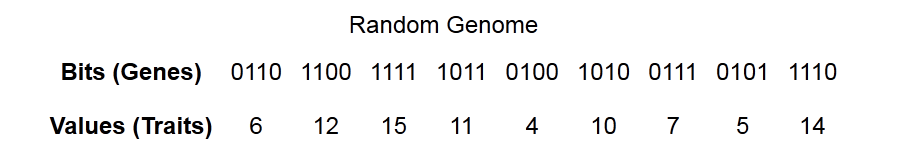
\includegraphics[scale=0.8]{genome.png}
	\caption{Random Genome}
	\label{fig:ID3}
\end{figure}


\subsection{Survival of the Fittest}
Every genome in the population must now be assigned a fitness score according to how well it solves the problem at hand. The process and approach to measuring a genome’s fitness will be different for every problem. Determining the fitness measure is the most important and often most difficult part of developing a genetic algorithm. 

\subsection{The Next Generation}

Once the fitness for every genome is determined, it’s time to start building the next generation of genomes based on probability and fitness. This is the main part of the genetic algorithm, where the strong survive and the weak perish. It usually consists of these three parts: 

\subsubsection{Selection}
Two genomes are selected randomly from the current population (reselection allowed), with fitter genomes having a higher chance of selection. The selected genomes, which should have a relatively high fitness score, are guaranteed to pass some of their traits to the next generation. This means that the average fitness of each successive generation will tend to increase.

The best way to program the selection function is through a method creatively named roulette selection. First, a random number between zero and the sum of the population’s fitness is generated. Imagine this value as a ball landing somewhere on a pie graph of the population’s fitness. Then, each genome’s fitness, or slice of the pie graph, is added one by one to a running total. If the ball ends up in that genome’s slice, it is selected. 

\begin{figure}[h!]
	\centering
		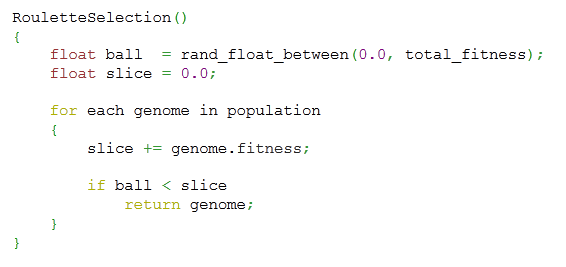
\includegraphics[scale=1.0]{roulette.png}
	\caption{Roulette Selection Pseudo-Code}
	\label{fig:ID3}
\end{figure}


\subsubsection{Crossover}
The two genomes now have a good chance of crossing over with one another, meaning that they will each donate a portion of their genes to form two offspring that become part of the next generation. If they do not cross over, they simply go on to the next generation unchanged. The crossover rate determines how often the genomes will cross over, and should be in the vicinity of 65-85%.

A crossover operation on the binary genomes in our example would begin by choosing a random position at which to cross them. The first part of the father’s genes and the second part of the mother\'s genes combine to form the first child, with a similar effect for the second child. The following shows a crossover operation with the crossover point at 12. 

\begin{figure}[h!]
	\centering
		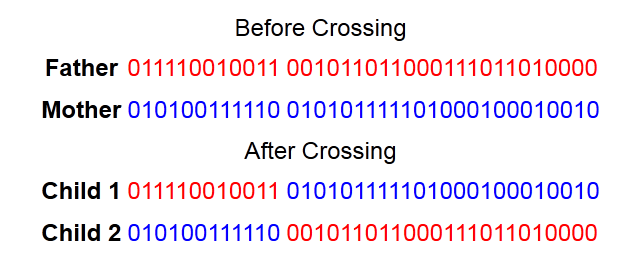
\includegraphics[scale=1]{crossover.png}
	\caption{Crossover}
	\label{fig:ID3}
\end{figure}


\subsubsection{Mutation}
Just before the genomes are placed into the next generation, they have a slight chance of mutating. A mutation is simply a small, random change to one of the genes. With binary genes, mutation means flipping the bit from 1 to 0 or 0 to 1. With real number genes, a small, random perturbation is added to the gene. 

\begin{figure}[h!]
	\centering
		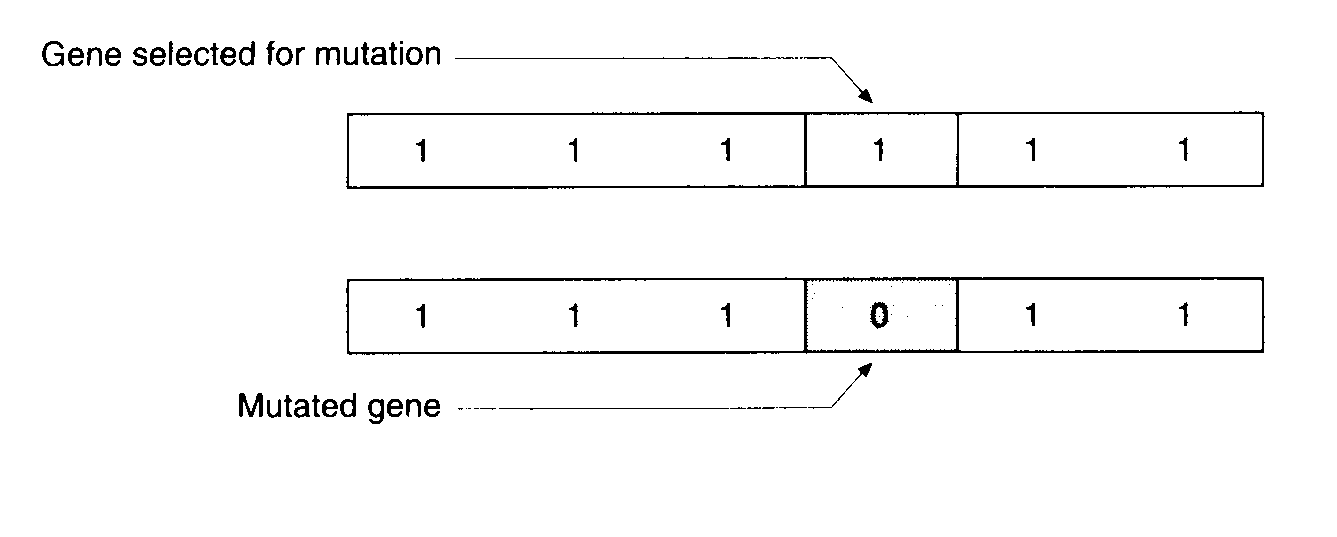
\includegraphics[scale=1.0]{mutation.png}
	\caption{Mutation}
	\label{fig:mutation}
\end{figure}

The mutation rate determines the chances for each gene to undergo mutation, meaning that every individual gene should get a chance to mutate. The mutation rate should be roughly 1-5 percent for binary and 5-20 percent for real numbers. 

The purpose of mutation in GAs is preserving and introducing diversity. Mutation should allow the algorithm to avoid local minima by preventing the population of chromosomes from becoming too similar to each other, thus slowing or even stopping evolution. This reasoning also explains the fact that most GA systems avoid only taking the fittest of the population in generating the next but rather a random (or semi-random) selection with a weighting toward those that are fitter.




\pagestyle{fancy}
\lhead{\scriptsize{Conclusion}}
\chead{}
\rhead{\scriptsize{DT classifier with GA based feature selection}}
\lfoot{\scriptsize{Dept. of CSE, R V C E, Bangalore.}}
\rfoot{\small{\thepage}}
\cfoot{\scriptsize{Sept 2012 - Jan 2013}}
\renewcommand{\headrulewidth}{0.4pt}
\renewcommand{\footrulewidth}{0.4pt}
\chapter{Decision Trees and Genetic Algorithms}
In GA based DT Classifier, the search component is a GA and the
evaluation component is a decision tree. A detailed description of
this algorithm is shown in Figure 5.1.

\begin{figure}[h!]  
  \centering
    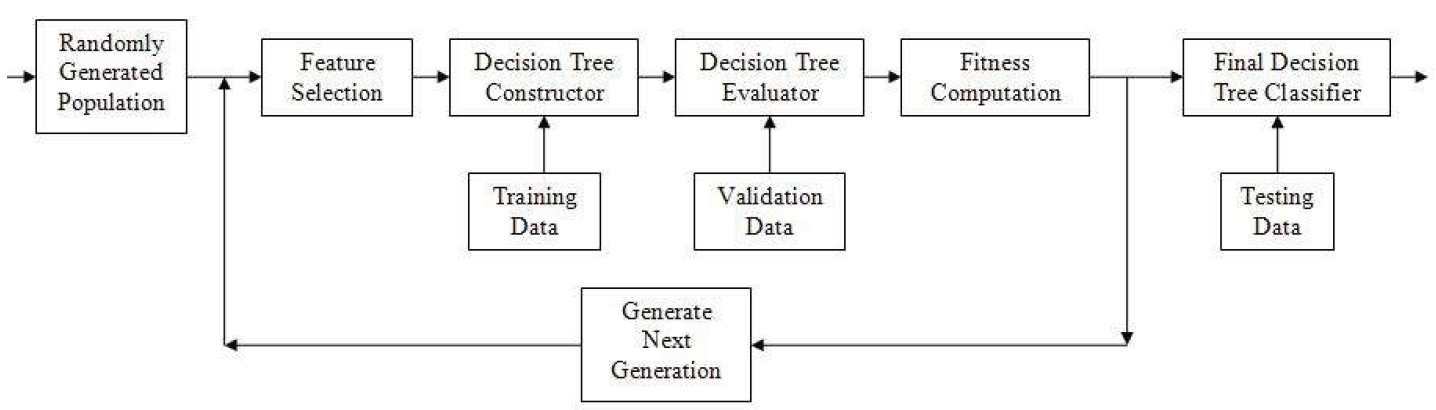
\includegraphics[scale=0.40]{dfd.png}
\caption{The data flow in DT/GA Hybrid Classifier Algorithm.}
\end{figure}

The basic idea of our hybrid system is to use GAs to
efficiently explore the space of all possible subsets of a given
feature set in order to find feature subsets which are of low
order and high discriminatory power. In order to achieve this
goal, fitness evaluation has to involve direct
measures of size and classification performance, rather than
measures such as the ranking methods such as information gain, etc.

An initial set of features is provided together with a training
set of the measured feature vectors extracted from raw data
corresponding to examples of concepts for which the decision
tree is to be induced. The genetic algorithm (GA) is used to
explore the space of all subsets of the given feature set where
preference is given to those features sets which achieve better
classification performance using smaller dimensionality feature
sets. Each of the selected feature subsets is evaluated (its
fitness measured) by testing the decision tree produced by the ID3 algorithm. The above process is iterated along evolutionary
lines and the best feature subset found is then recommended to
be used in the actual design of the pattern classification
system.


\section{Representation of Chromosomes}
Every individual of the population has N genes, each of which represents a feature of the input data and can be assigned to 1 or 0. 
1 means the represented feature is used during constructing decision trees; 0 means it is not used. As a result, each individual in the population represents a choice of available features. 

\begin{figure}[h!]  
  \centering
    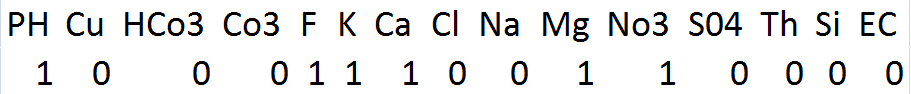
\includegraphics[scale=0.70]{featurechromosome.png}
\caption{Sample Representation}
\textit{In this figure, only the following features are being considered: PH, F, K, Ca, Mg, and No3, yielding the chromosome: 100011100110000}
\end{figure}


\section{Population}
The initial population is randomly generated. For each individual in the current population, a decision tree is built using the ID3 algorithm. This resulting decision tree is then tested over validation data sets, which generate classification error rates. In our application, we calculate fitness values using the weighted average of training and test classification errors. The lower the classification error rate, the better the fitness of the
individual. In other words, the population consists of a number of probable decision trees.

\section{Advantages}
Such a hybrid learning system will identify significantly better feature subsets than those produced by existing methods for two reasons. 
\begin{enumerate}
\item{The power of Genetic algorithms is being exploiting to efficiently explore the non-linear interactions of a given set of features.}
\item{By using ID3 in the evaluation loop, an efficient mechanism for directly measuring classification accuracy is present}

\end{enumerate}


\pagestyle{fancy}
\lhead{\scriptsize{Conclusion}}
\chead{}
\rhead{\scriptsize{DT Classifier with GA based feature selector.}}
\lfoot{\scriptsize{Dept. of CSE, RVCE, Bangalore.}}
\rfoot{\small{\thepage}}
\cfoot{\scriptsize{Sept 2012 - Jan 2013}}
\renewcommand{\headrulewidth}{0.4pt}
\renewcommand{\footrulewidth}{0.4pt}
\chapter{Our State-of-the-art Object-Oriented System}

Object-oriented programming (OOP) is a programming paradigm that represents concepts as "objects" that have data fields \textit{(attributes that describe the object)} and associated procedures known as methods. Objects, which are instances of classes, are used to interact with one another to design applications and computer programs.
\\Had it not been for the presence of the OOP paradigm, our efforts in this project would have gone in vain, and we do not use that term lightly. Code management was a whole lot easier when compared to our past experience with procedural programming. In this chapter, we describe the different packages that were created by us to efficiently manage our code. Know first that our application consists of four diverse packages, namely:\textbf{
\begin{enumerate}
\itemsep-0.5em
\item{org.ck.sample}
\item{org.ck.dt}
\item{org.ck.ga}
\item{org.ck.gui}
\end{enumerate}}


We describe each package in detail, in the following sections. We follow a bottom-up methodology for explaining the layout of the classes.

\section{org.ck.sample}
This package allows us to efficiently manage and encapsulate the details of the data samples, provided by users, which are required for analysis. It is this class that allows our application to accept generic data sets. It consists of five classes:

\begin{enumerate}
\item{\textbf{DataHolder}} - This class keeps track of names of files that contain training and testing samples; lists of features; their corresponding classification values; and Probability values. It provides this information, when required, to the front-end or back-end of our application. To make a long story short, this class acts like a middleman between the back-end and front-end of our application.
\item{\textbf{Feature}} - This class stores a mapping between a feature name and a feature value.

\item{\textbf{Sample}} - This class stores all the features and the corresponding classification value for one training/test sample only.  

\item{\textbf{SampleCollection}} - A SampleCollection, as the name suggests, is a collection of samples. In essence, this class reads the sample data from a file (using information provided by a DataHolder object) and initializes all the necessary data structures to store the data values for Classification analysis.

\item{\textbf{SampleSplitter}} - This class contains methods that operate on a given SampleCollection, in order to split it into two new SampleCollections, based on a given Feature. It also calculates the information gain \textit{(as described in Chapter 3)} of the given split operation.


\end{enumerate}



\section{org.ck.dt}

This package allows us to efficiently manage and encapsulate methods for all stages of Decision Tree Learning.

\begin{enumerate}

\item{\textbf{DecisionTreeNode}} - A DecisionTreeNode is a structure which may have either:

\begin{enumerate}
\item{a classification value, if it happens to be a leaf node}
\item{a list of one or more children DecisionTreeNodes, if it happens to be a decision node, i.e., an internal node.}
\end{enumerate}

Know that the types of these nodes is defined by the decision tree that is constructed, and a node has at most one parent.

\item{\textbf{DecisionTreeConstructor}} - This class takes a SampleCollection \textit{(containing training samples)} as input,  builds a decision tree \textit{(as described in Chapter 3)} and stores the root DecisionTreeNode of the decision tree. In essence, a DecisionTreeConstructor consists of a number of DecisionTreeNodes.

\item{\textbf{DecisionTreeClassifier}} - This class keeps track of the measurements of the DecisionTree constructed by a DecisionTreeConstructor object. It keeps track of the training as well as the test SampleCollection, and runs each sample through the Decision Tree that was constructed, to find out its classification accuracy, which it stores and retrieves, when required.


\item{\textbf{Discretizer}} - This class provides implementations of algorithms used for discretization. As mentioned earlier, decision trees work with discretized values, and if continuous-valued features are present, they have to be discretized. The Discretizer class contains two algorithms for discretization:
\begin{enumerate}
\item{A naive discretizer that discretizes data based on the median, with those values below the median being set to 0 and those values above the median being set to 1.}
\item{An Equal-Binning Discretizer that discretizes the values of certain feature of a collection of samples, by putting each value into particular bins. After discretization, the values can be any integer between 0 and binSize (inclusive).}
\end{enumerate}

\end{enumerate}








\section{org.ck.ga}
This package takes care of all operations of the Genetic algorithm that was mentioned earlier.

\begin{enumerate}
\item{\textbf{Genome}} - This class takes as input, a SampleCollection, and initializes a chromosome with random values for the presence/absence of features, as defined in Chapter 5. It keeps track of this chromosome, and provides methods to manipulate this chromosome; to calculate the fitness score of this chromosome; and to throw an exception when the fitness value threshold has been crossed or when the best solution has been discovered. It also provides facilities to switch between a chromosome and the corresponding optimal decision tree to which it is bound.


\item{\textbf{Population}} - As defined earlier, a population is a collection of genomes. And this is exactly what this class is. Initially, the Population class randomly initializes a large number of genomes, of which it keeps track. It provides methods such as roulette selection, reproduction, crossover, and mutation to operate on the population and discover the best genome, and hence, the best decision tree with the appropriate feature subset.

\item{\textbf{OptimalScoreException}} - This class is responsible for catching the best genome as soon as it is discovered, since the best genome should never be allowed to escape. It should be caught and nurtured for future use.

\end{enumerate}


\section{org.ck.gui}

As you've probably guessed by now, this package handles the Graphical User Interface of our application, with all its bells and whistles. We made use of the Standard Widget Toolkit for the GUI of our application. This package consists of the following classes:

\begin{enumerate}

\item{\textbf{WelcomeWindow}} - This class takes care of drawing the window that appears when our application is first switched on, and obviously, its name should be WelcomeWindow, nothing more, nothing less. It displays a list of clickable options, namely
\begin{enumerate}
\item{Train Decision Tree}
\item{Classify Data Sets}
\item{View on Github}
\item{Exit Application}
\end{enumerate}

We have organized the code in this package in such a way that all the options \textit{(except for the last one - "Exit Application")}, correspond to a different class which handles the creation of the corresponding window.

\item{\textbf{MainWindow}} - This class manages the window that is opened when a user clicks the \textit{Train Decision Tree} option in the Welcome Window. In this window, the user can select the appropriate options required to construct a decision tree using our Hybrid DT/GA Classifier. By the way, did we mention that a constructed decision tree can be saved for later usage?

\item{\textbf{ClassifyWindow}} - This class manages the window that is opened when a user clicks the \textit{Classify Data Sets} option in the Welcome Window. A user is provided with an interface to select a saved decision tree, and classify new samples based on it. It really saves a lot of time in this fast-paced world of ours.


\item{\textbf{BrowserWindow}} - This class manages the window that is opened when a user clicks the \textit{View on Github} option in the Welcome Window. In order to see and verify whether our code is original or not, users can see the online repository of our code (including its version history) on Github, in this window. Verification couldn't have been more easier. 

\item{\textbf{Constants}} - This interface (mark my words, this is not a class) contains a list of constants used by all the classes in all the packages. This interface really makes updating our software and meddling with various values much easier, like never before.



\item{\textbf{MainClass}} - Before our application had a GUI, this class was used to test out the code in the other packages using the console. The SampleCaller2 method is still being used by the MainWindow class. We didn't have the heart to delete this class, which has been with us for so very long. We kept it for old times' sake.



\end{enumerate}






\pagestyle{fancy}
\lhead{\scriptsize{Conclusion}}
\chead{}
\rhead{\scriptsize{DT Classifier with GA based feature selector.}}
\lfoot{\scriptsize{Dept. of CSE, RVCE, Bangalore.}}
\rfoot{\small{\thepage}}
\cfoot{\scriptsize{Sept 2012 - Jan 2013}}
\renewcommand{\headrulewidth}{0.4pt}
\renewcommand{\footrulewidth}{0.4pt}
\chapter{CONCLUSION AND FUTURE WORK}

\section{Summary}
In this mini project, we were able to successfully implement and test the performance of Decision Tree-based classifiers. The Decision Tree classifier was optimized using a Genetic Algorithm to select a subset of the features that were to be used in constructing an optimal decision tree.


Although our program works with generic data samples, it must be noted that when we started this project, our main intention was to classify ground water samples into two classes, namely Potable and Non-Potable Water. However, thanks to the miracle of Object-Oriented Programming Concepts, we were able to extend our application, which was developed in Java and Java SWT. We were able to extend this application to work with any generic samples. Two other samples/ Classification problems were addressed:
\begin{itemize}
\item{Diagnosing whether a Horse has colic or is healthy, based on its Blood Sample Data.}
\item{Classifying/Determining the quality of a wine based on Data Samples containing it\'s quality parameters} 
\end{itemize} 

The hybrid GA /decision tree algorithm needs to be tested
further to realize its true potential. Clearly more work needs to be done. 
The test results show that the Decision Trees constructed using the Genetic algorithm-based feature selector, were more efficient and accurate in classifying the data than the Decision Trees constructed by selecting features manually.

\section{Limitations}
These are a few limitations of this application.
\begin{enumerate}
\item{The application uses about 800MB-1GB of RAM.}

\item{The GA feature selector takes a considerable amount time to optimize the Decision Tree depending on the size of the training and testing samples.}
\item{The GA optimizer may take a long time to converge or may not converge at all, which usually results in the application crashing, due to high memory usage.}
\item{ The Decision Tree classifier with GA-based feature selection requires the use of accurate as well as a large number of training and testing samples. The efficiency of the Decision Tree constructed is solely based on the input training and testing samples.}

\end{enumerate}
\section{Future enhancements}
Some of the future enhancements are :
\begin{enumerate}
\item{The application could be made more responsive by using Threads and Parallel/Cloud Computing}
\item{The Decision Tree Classifier of this application could be optimized using Neural Networks which are more efficient than Decision Trees.}
\item{An interesting extension to be explored is the possibility of
additional feedback from ID3 concerning the evaluation of a
feature set. Currently only classification accuracy is returned.
However, there is potentially exploitable information with
respect to which features were actually used to build the
decision tree and their relative positions in the tree.}

\end{enumerate}

\newpage

%For Bib refer to refs.bib to add/remove bib items
\addcontentsline{toc}{section}{BIBLIOGRAPHY}
\begin{thebibliography}{refs}
\bibitem{test}Genetic Algorithms  -\url{http://en.wikipedia.org/wiki/Genetic_algorithm}
\bibitem{t}Genetic Algorithm for constructing DT - \url{http://www.jprr.org/index.php/jprr/article/viewFile/44/25}
%\bibtitem{te}Decision Trees - \url{http://web.cecs.pdx.edu/~mm/MachineLearningWinter2010/pdfslides/DecisionTrees.pdf}
\bibitem{t} Project brief for the DT  using Horse data sets  - \url{https://cs.uwaterloo.ca/~ppoupart/teaching/cs486-spring06/assignments/asst4/asst4.pdf}
\bibitem{t}Supervised and Unsupervised Discretization of Continous Features - \url{http://robotics.stanford.edu/users/sahami/papers-dir/disc.pdf}
\bibitem{t}Hybrid learning using Genetic Algorithms and Decision Trees for pattern sification - \url{http://cs.gmu.edu/~eclab/papers/ijcai95.pdf}
\bibitem{t}Kardi Maams' Tutorials - \url{http://people.revoledu.com/kardi/tutorial/DecisionTree/index.html}

%\bibitem{}
%\bibitem{}
\end{thebibliography}

\newpage
\pagestyle{fancy}
\lhead{\scriptsize{Appendix A: Source Code}}
\chead{}
\rhead{\scriptsize{DT Classifier with GA based feature selector.}}
\lfoot{\scriptsize{Dept. of CSE, RVCE, Bangalore.}}
\rfoot{\small{\thepage}}
\cfoot{\scriptsize{Sept 2012 - Jan 2013}}
\renewcommand{\headrulewidth}{0.4pt}
\renewcommand{\footrulewidth}{0.4pt}

\addcontentsline{toc}{section*}{APPENDICES}
\section*{Appendices}
\section*{Appendix A : Source Code}

\lstinputlisting[language=Java, caption=DataHolder.java, breaklines=true]{../src/org/ck/sample/DataHolder.java}
\lstinputlisting[language=Java, caption=Feature.java, breaklines=true]{../src/org/ck/sample/Feature.java}
\lstinputlisting[language=Java, caption=Sample.java, breaklines=true]{../src/org/ck/sample/Sample.java}
\lstinputlisting[language=Java, caption=SampleCollection.java, breaklines=true]{../src/org/ck/sample/SampleCollection.java}
\lstinputlisting[language=Java, caption=SampleSplitter.java, breaklines=true]{../src/org/ck/sample/SampleSplitter.java}

\lstinputlisting[language=Java, caption=DecisionTreeNode.java, breaklines=true]{../src/org/ck/dt/DecisionTreeNode.java}
\lstinputlisting[language=Java, caption=DecisionTreeConstructor.java, breaklines=true]{../src/org/ck/dt/DecisionTreeConstructor.java}
\lstinputlisting[language=Java, caption=DecisionTreeClassifier.java, breaklines=true]{../src/org/ck/dt/DecisionTreeClassifier.java}
\lstinputlisting[language=Java, caption=Discretizer.java, breaklines=true]{../src/org/ck/dt/Discretizer.java}

\lstinputlisting[language=Java, caption=Genome.java, breaklines=true]{../src/org/ck/ga/Genome.java}
\lstinputlisting[language=Java, caption=Population.java, breaklines=true]{../src/org/ck/ga/Population.java}
\lstinputlisting[language=Java, caption=OptimalScoreException.java, breaklines=true]{../src/org/ck/ga/OptimalScoreException.java}

\lstinputlisting[language=Java, caption=WelcomeWindow.java, breaklines=true]{../src/org/ck/gui/WelcomeWindow.java}
\lstinputlisting[language=Java, caption=MainWindow.java, breaklines=true]{../src/org/ck/gui/MainWindow.java}
\lstinputlisting[language=Java, caption=ClassifyWindow.java, breaklines=true]{../src/org/ck/gui/ClassifyWindow.java}
\lstinputlisting[language=Java, caption=BrowserWindow.java, breaklines=true]{../src/org/ck/gui/BrowserWindow.java}
\lstinputlisting[language=Java, caption=MainClass.java, breaklines=true]{../src/org/ck/gui/MainClass.java}
\lstinputlisting[language=Java, caption=Constants.java, breaklines=true]{../src/org/ck/gui/Constants.java}


%\begin{lstinputlisting}[label=some-code,caption=Some Code]{Charnode.h}
%\lstinputlisting[ language=C++, label=charnode, caption=The definiton of the class Charnode\, each node of the huffman tree is an object of this class.]{Charnode.h}
%
%\lstinputlisting[language=C++, label=huffman,caption=The definition  of the class Huffman\, this class helps in building the huffman tree for an input file.]{HuffmanCode.h}
%
%\lstinputlisting[language=C++, label=compresswrite,caption=The definition  of the class CompressionWriting\, this class helps in writing the bits to the compressed file.]{CompressionWriting.h}
%
%\lstinputlisting[language=C++, label=huff,caption=The main program of the huffman compression algorithm.]{huff.cpp}
%
%\lstinputlisting[language=C++, label=unhuff,caption=The definition of the class Decompressor\, this class helps in decompressing the compressed file using huffman algorithm.]{Decompressor.h}
%
%\lstinputlisting[language=C++, label=unhuff,caption=The main program of the huffman decompression algorithm.]{unhuff.cpp}


%\lstinputlisting[language=C++, label=unhuff,caption=The definition of the class TCP\_Server\, an object of this class is a server object that can concurrently handle requests for files from the clients.]{TCP_Server.h}

%\lstinputlisting[language=C++, label=unhuff,caption=The definition of the class TCP\_Client\, an object of this class indicates a client object that can request for files from the server.]{TCP_Client.h}


\newpage
\pagestyle{fancy}
\lhead{\scriptsize{Appendix B: Screen shots}}
\chead{}
\rhead{\scriptsize{DT Classifier with GA based feature selector.}}
\lfoot{\scriptsize{Dept. of CSE, RVCE, Bangalore.}}
\rfoot{\small{\thepage}}
\cfoot{\scriptsize{Sept 2012 - Jan 2013}}
\renewcommand{\headrulewidth}{0.4pt}
\renewcommand{\footrulewidth}{0.4pt}


\section*{Appendix B : Screen Shots}
\begin{figure}[h!]

  \centering
    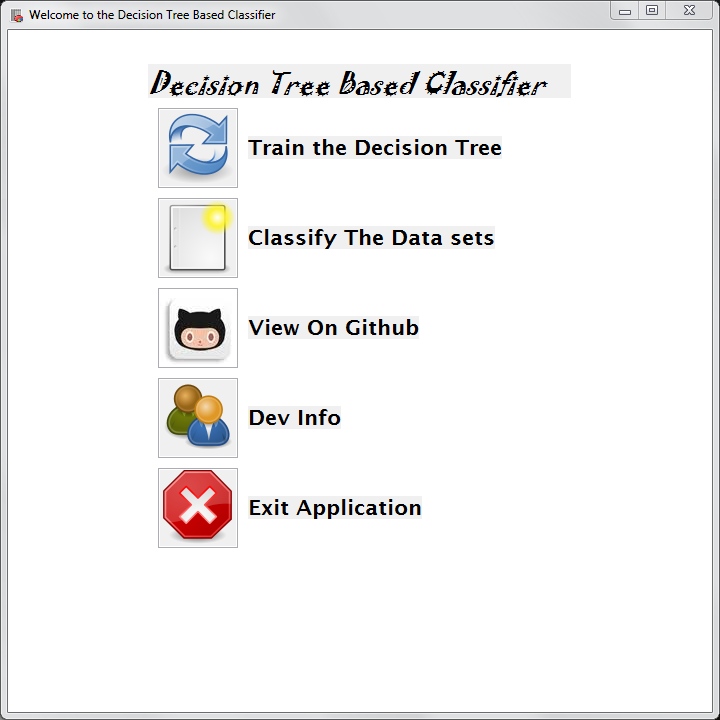
\includegraphics[scale=0.40]{welcome_window.png}
  \caption{Application Window - Welcome Screen}
\end{figure}

\begin{figure}[h!]
  
  \centering
    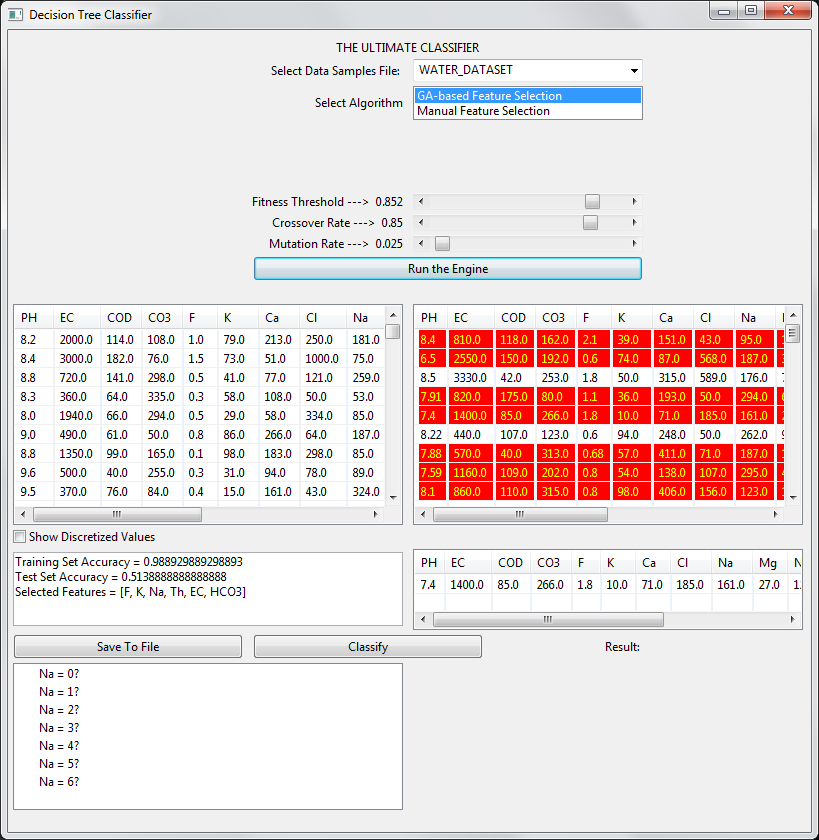
\includegraphics[scale=0.45]{dt_classifier.png}
\caption{Decision Tree Constructor Window.}
\end{figure}

\begin{figure}[h!]
  
  \centering
    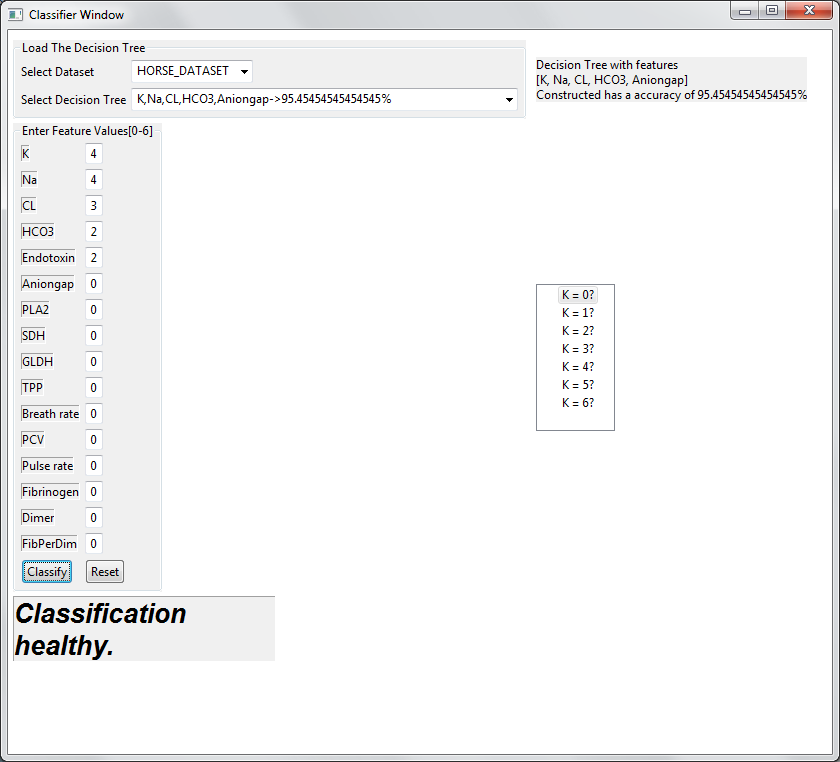
\includegraphics[scale=0.45]{dt_classification_window.png}
\caption{Decision Tree Classifier Window.}
\end{figure}
\begin{figure}[h!]
  
  \centering
    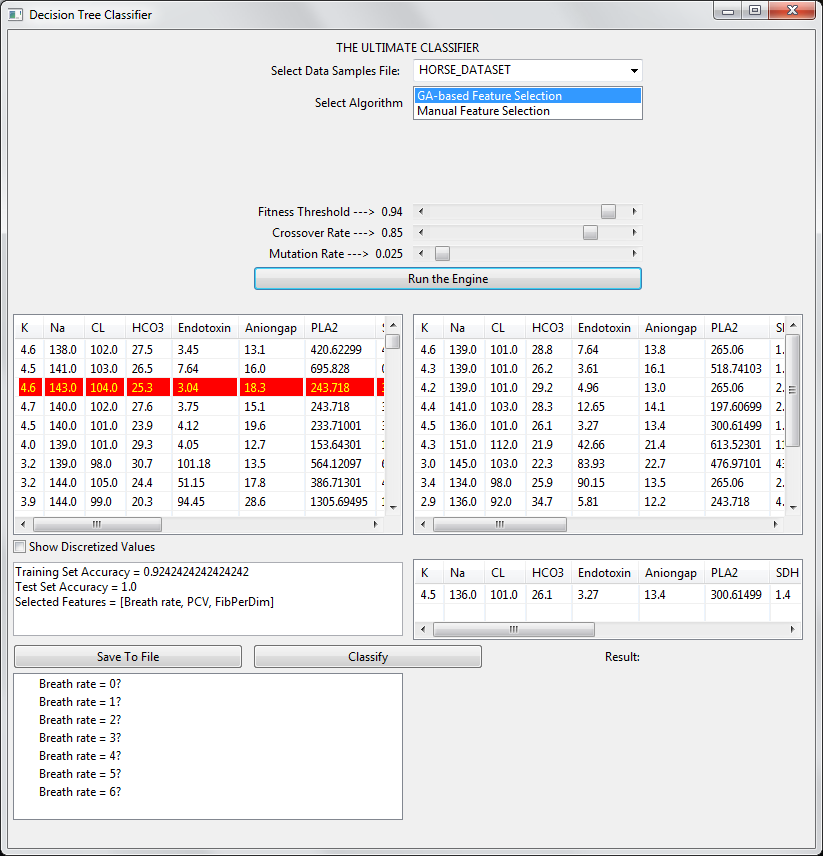
\includegraphics[scale=0.45]{dt_ga_algorithm.png}
\caption{Decision Tree Construction with GA based Feature Selector.}
\end{figure}

\begin{figure}[h!]
  
  \centering
    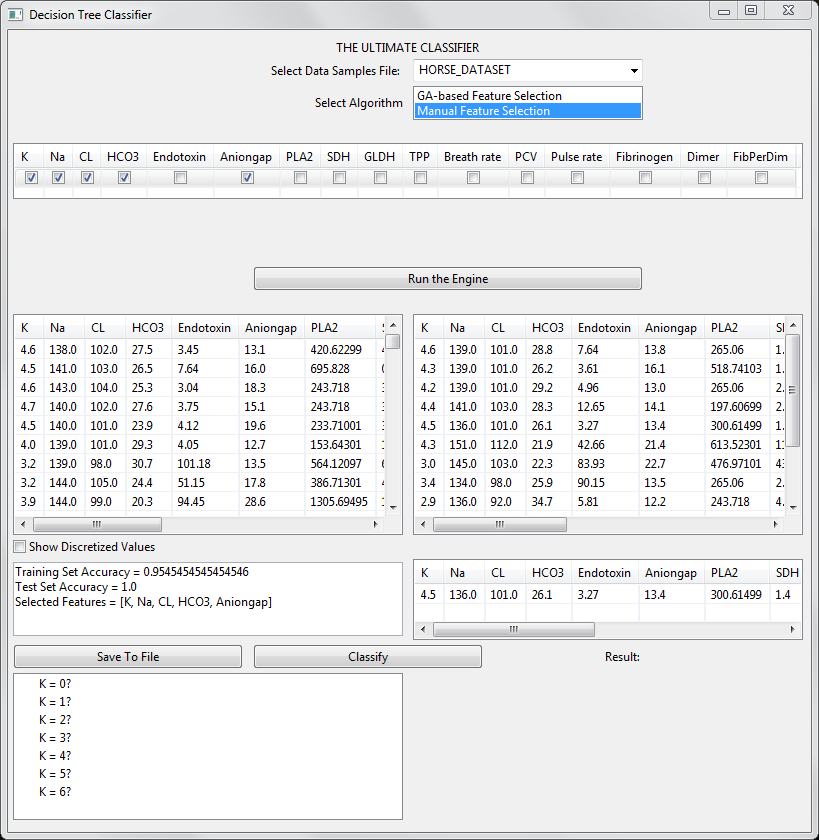
\includegraphics[scale=0.45]{dt_manual_selection.png}
\caption{Decision Tree Construction with manual feature selection.}
\end{figure}

\begin{figure}[h!]
  
  \centering
    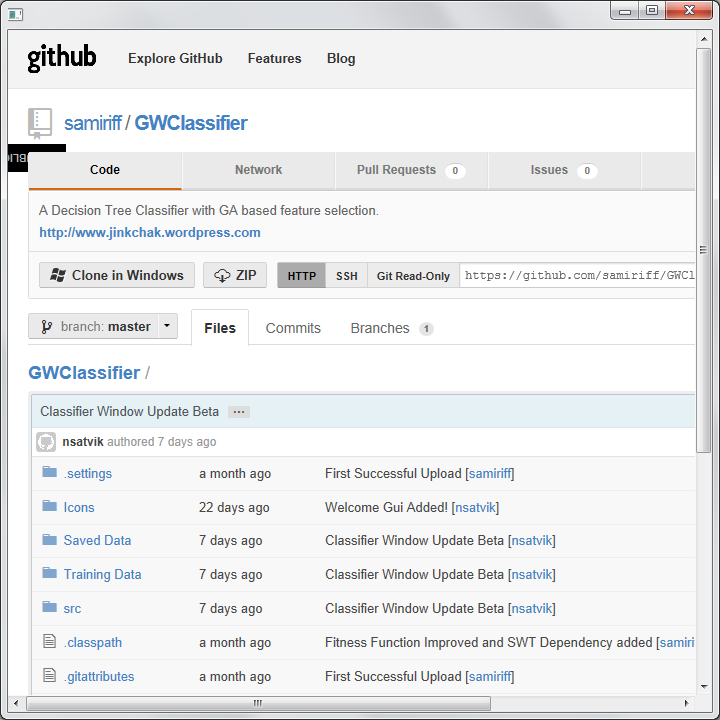
\includegraphics[scale=0.45]{git_hub.png}
\caption{The project source code on github public repository.}
\end{figure}


\end{document}
